Phytoplankton are primary producers and base of the food chain.
The distribution of phytoplankton biomass and net primary production is defined by the availability of light and nutrients (nitrogen, phosphate, iron). 
These growth-limiting factors are in turn regulated by physical processes of ocean circulation, 
mixed-layer dynamics, upwelling, atmospheric dust deposition, and the solar cycle.\supercite{ref1}

Phytoplankton blooms are sudden increases in phytoplankton concentration. 
The timing of these blooms plays an important role in maintaining marine ecosystems. 
However, there are also harmful phytoplankton blooms bringing death or disease killing marine life, 
because certain species of phytoplankton produce powerful biotoxins.\supercite{ref2}

To understand the initiation of phytoplankton blooms it is important to be familiar with the concepts euphotic zone depth (EZD), 
mixed layer depth (MLD), critical depth and compensation depth. 

The ocean is divided into three zones based on depth and light level. 
The upper zone is called the euphotic, or "sunlight," zone. Ninety percent of marine life lives in this zone. 
Only a small amount of light penetrates beyond this depth where the dysphotic zone and the aphotic zone exist. 
The depth of the euphotic zone (EZD) depends on the transparency of the water (Fig 1).\supercite{ref3}

Fig 1. The euphotic, dysphotic and aphotic zones\supercite{ref fig1}
The surface mixed layer is the layer between the ocean surface and the depth defined as mixed layer depth, MLD, where salinity, temperature, and density are almost vertically uniform. 
In the open ocean the mixed layer is usually ranging between 25 and 200m. 
It exists due to the mixing initiated by waves and turbulence caused by the wind stress on the sea surface and mostly depends on the stability of the sea water and on the incoming energy from the wind. 
The more stable is the surface water, the less mixing occurs, and the shallower is the mixed layer.\supercite{ref4}

Compensation depth is the depth where the rate of photosynthesized organic matter is equivalent to the rate of decomposed organic matter by plant respiration. 
The critical depth is the depth where solar radiation can just balance radiation (Fig2).\supercite{ref5} 


Fig 2. The relationship between the water depth, net primary production (NPP=P-R) and available sunlight explaining compensation depth and critical depth\supercite{ref fig2}


Phytoplankton blooms can be studied by using land-based and ship-based equipment for water samples and monitoring, 
long term moored boys, satellite instruments and unmanned underwater vehicles.\supercite{ref6}
Unmanned underwater vehicles can be remotely operated underwater vehicles (ROVs) and autonomous underwater vehicle (AUV), 
which is a robot travelling underwater without requiring input from an operator.  
AUV:s have recently become an attractive alternative for underwater research and exploration since they are cheaper than manned vehicles. 
Gliders are underwater autonomous buoyance-driven vehicles capable of remaining at sea for long periods of time while continuously collecting data from a range of disciplines at high resolution. 
It has its advantages with lower costs compared to other ways of collecting data, 
still with high accuracy, but there are occasionally difficulties with the equipment and the control of it. 
There are also other factors affecting and restricting the use of them; 
this includes interfering with shipping and fishing as well as the difficulty obtaining state and international permits.

This study analysis the evolution of phytoplankton through blossom in the Bornholm basin using data collected by gliders within the infrastructure project Smart Autonomous Monitoring of the Baltic Sea (SAMBA) funded by the Voice of the Ocean Foundation.\supercite{ref7}
The mission and purpose of the Voice of the Ocean Foundation, run by a group of oceanographers, historians and entrepreneurs, 
is to “conduct, support and promote science, education, information and communication regarding the sea, marine ecosystems, 
and the marine environment as well as the interaction between man and the sea, historically, at the present time and in the future.”\supercite{ref8} 

The observations are run by a group of oceanographers, technicians and a piloting team since March 2021 on two locations, Skagerrak and in the Bornholm basin. 
The project combines short term science objectives and a long-term vision of establishing several persistent ocean observatories across the Baltic Sea for international collaboration.\supercite{ref7}

The focus area in this report is the Bornholm basin, which is in southwest of the Baltic Sea (Fig 3).


Fig 3. The location of the Bornholm Basin and its water depths\supercite{ref fig3}


This study analyses some of these glider data, giving insight into two phytoplankton blooms occurring during the period March to October 2021, 
as a project part of the course MAR440 Marine Project from idea to realization at University of Gothenburg the autumn 2021.


References

Ref 1
Behrenfeld, M., O’Malley, R., Siegel, D. et al.Climate-driven trends in contemporary ocean productivity. Nature 444, 752–755 (2006). https://doi.org/10.1038/nature05317
Ref 2
Theodore J. Smayda, What is a bloom? A commentary First published: 22 December 2003
https://doi.org/10.4319/lo.1997.42.5_part_2.1132
Limnol,  Oceanogr,  42(5, part  2 Bloom, dynamics:Physiolocy, behavior, trophic),  1997,  1132-1136  1997,  by  the  American  Society  of  I,imnology and  Occaoography,  Inc.
Ref 3
https://oceanservice.noaa.gov/facts/light_travel.html

Ref 4
Clément de Boyer Montégut,Gurvan Madec,Albert S. Fischer,Alban Lazar,Daniele Iudicone,
Mixed layer depth over the global ocean: An examination of profile data and a profile-based climatology
First published: 04 December 2004
https://doi.org/10.1029/2004JC002378


Ref 5
(ref 8 according to already used reference in report – Harald Erik Sverdrup
Ref 6
Davis et al., 2019
R.E. Davis, L.D. Talley, D. Roemmich, B. Owens, D.L. Rudnick, J. Toole, R. Weller, M.J. McPhadden, J.A. Barth
100 Years of progress in ocean observing systems
Meteorol. Monogr. (2019), 10.1175/AMSMONOGRAPHS-D-18-0014.1
Google Scholar


Ref 7
https://voiceoftheocean.org/
retrieved 2021 10 18
Ref 8
Bastien Queste, Sebastiaan Swart, Louise Biddle, Olle Petersson, Aleksandra Mazur, et al.. OBSERVING BALTIC SEA EXCHANGES: PRESENTING A NEW MULTI-PLATFORM AUTONOMOUS OBSERVATORY. 9th EuroGOOS International conference, Shom; Ifremer; EuroGOOS AISBL, May 2021, Brest, France. ?hal-03331198v2?

Fig 1
https://oceanservice.noaa.gov/facts/light_travel.html

Fig 2
ecology - The effect of depth on net primary production in aquatic ecosystems - Biology Stack Exchange
https://biology.stackexchange.com/questions/54215/the-effect-of-depth-on-net-primary-production-in-aquatic-ecosystems
retrieved 2021 10 20

Fig 3
Hinrichsen H.-H., von Dewitz B., Dierking J., Haslob H., Makarchouk A., Petereit C., Voss R.
Oxygen depletion in coastal seas and the effective spawning stock biomass of an exploited fish speciesR. Soc. open sci.3150338150338,  2016
http://doi.org/10.1098/rsos.150338







\documentclass[../Main.tex]{subfiles}

\begin{document}
\section*{\crule[blue]{.3cm}{.3cm} Introduction}
Phytoplankton are primary producers and base of the food chain. 
The distribution of phytoplankton biomass and net primary production is defined by the availability of light and nutrients (nitrogen, phosphate, iron). 
These growth-limiting factors are in turn regulated by physical processes of ocean circulation, mixed-layer dynamics, upwelling, atmospheric dust deposition, and the solar cycle.\supercite{}

Phytoplankton blooms are sudden increases in phytoplankton concentration. 
The timing of these blooms plays an important role in maintaining marine ecosystems. 
However, there are also harmful phytoplankton blooms bringing death or disease killing marine life, 
because certain species of phytoplankton produce powerful biotoxins.\supercite{}

To understand the initiation of phytoplankton blooms it is important to be familiar with the concepts euphotic zone depth (EZD), mixed layer depth (MLD), 
critical depth and compensation depth. 

The ocean is divided into three zones based on depth and light level. 
The upper zone is called the euphotic, or "sunlight," zone. 
Ninety percent of marine life lives in this zone. 
Only a small amount of light penetrates beyond this depth where the dysphotic zone and the aphotic zone exist. 
The EZD depends on the transparency of the water.\supercite{}

\begin{figure}[H]
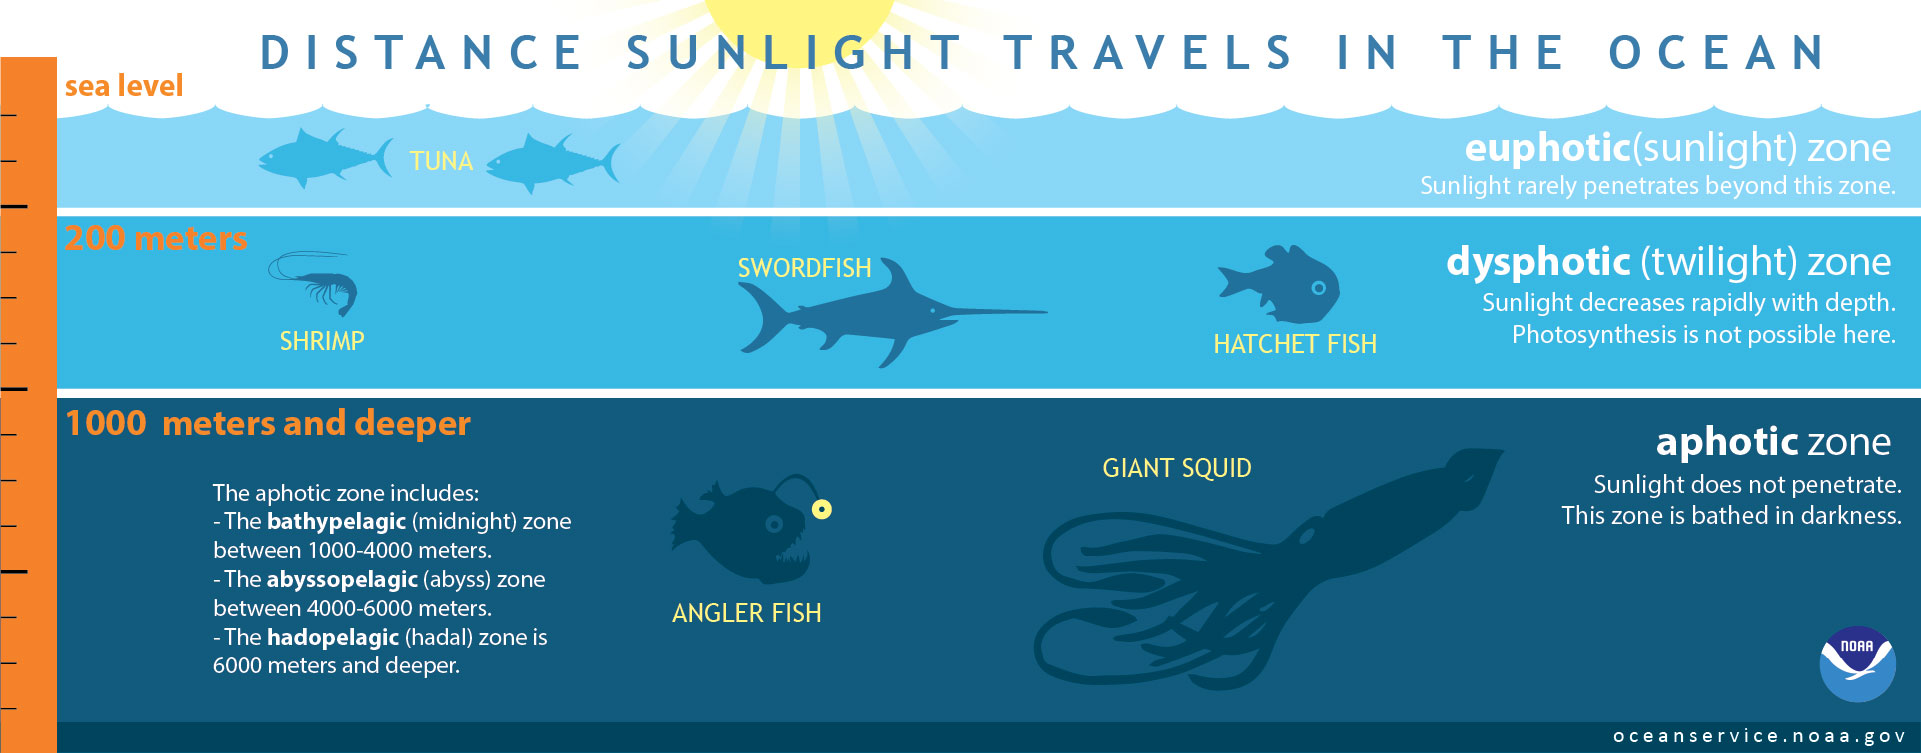
\includegraphics[width=0.5\textwidth]{EZD.jpg}
\caption{ The euphotic, dysphotic and aphotic zones.\supercite{}}
\end{figure}
The surface mixed layer is the layer between the ocean surface and the depth defined as mixed layer depth, MLD, 
where salinity, temperature, and density are almost vertically uniform. 
In the open ocean the mixed layer is usually ranging between 25 and \SI{200}{m}. 
It exists due to the mixing initiated by waves and turbulence caused by the wind stress on the sea surface and mostly depends on the stability of the sea water and on the incoming energy from the wind. 
The more stable is the surface water, the less mixing occurs, and the shallower is the mixed layer.\supercite{}

Compensation depth is the depth where the rate of photosynthesized organic matter is equivalent to the rate of decomposed organic matter by plant respiration. 
The critical depth is the depth where solar radiation can just balance radiation.\supercite{}

\begin{figure}[H]
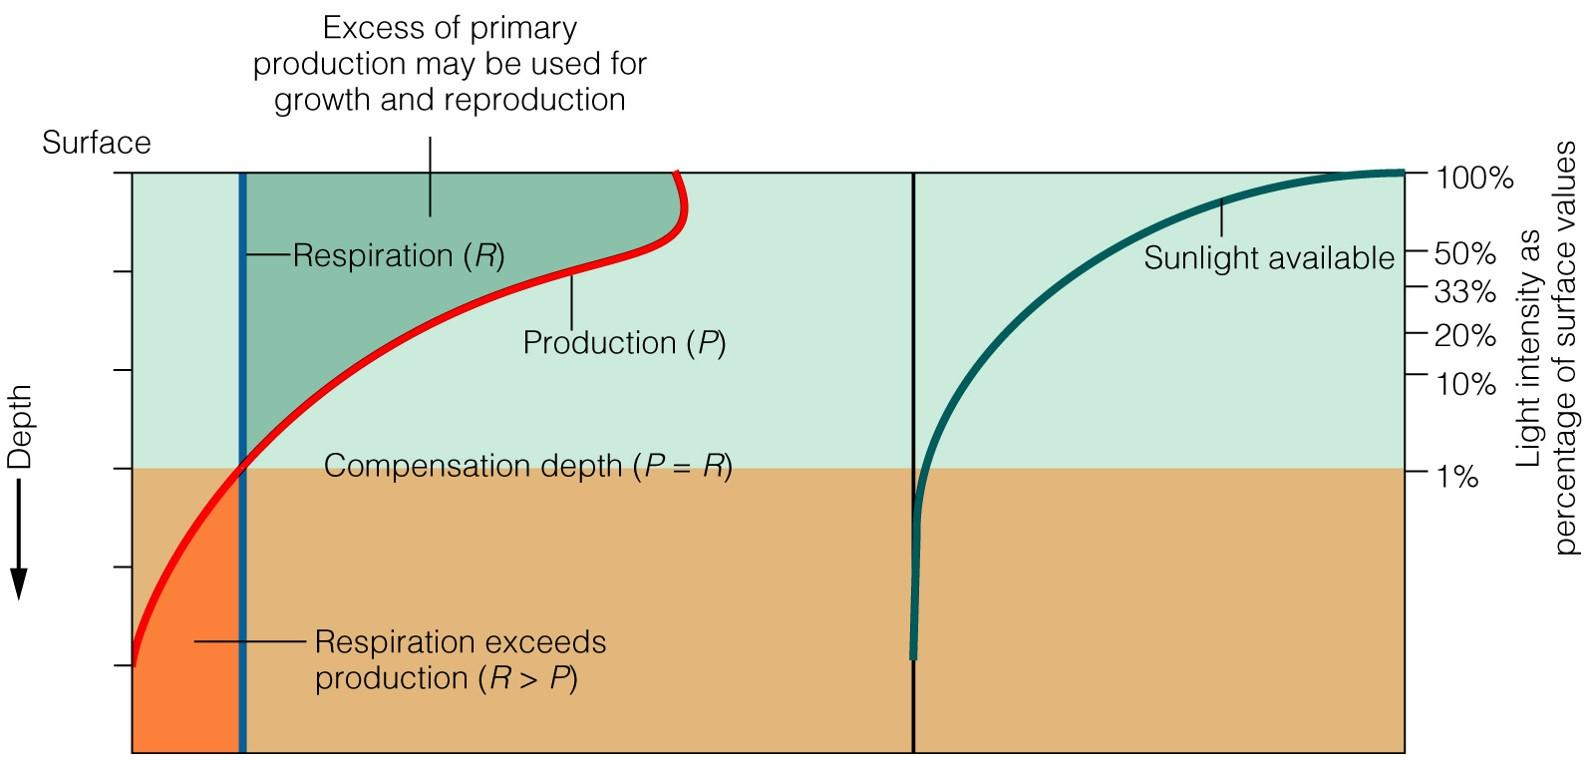
\includegraphics[width=0.5\textwidth]{Primary_Production.jpg}
\caption{ The relationship between the water depth and net primary production (NPP=P-R).\supercite{}}
\end{figure}

Phytoplankton blooms can be studied by using land-based and ship-based equipment for water samples and monitoring, long term moored boys, satellite instruments and unmanned underwater vehicles.\supercite{}
Unmanned underwater vehicles can be remotely operated underwater vehicles (ROVs) and autonomous underwater vehicle (AUV), 
which is a robot travelling underwater without requiring input from an operator. 
AUVs have recently become an attractive alternative for underwater research and exploration since they are cheaper than manned vehicles. 
Gliders are underwater autonomous buoyance-driven vehicles capable of remaining at sea for long periods of time while continuously collecting data from a range of disciplines at high resolution. 
It has its advantages with lower costs compared to other ways of collecting data, still with high accuracy, but there are occasionally difficulties with the equipment and the control of it. 
There are also other factors affecting and restricting the use of them; this includes interfering with shipping and fishing as well as the difficulty obtaining state and international permits

Gliders were used in collecting data for this study, which is analysing the evolution of phytoplankton through blooms in the Bornholm basin. 
The data was collected within the infrastructure project Smart Autonomous Monitoring of the Baltic Sea (SAMBA) funded by the Voice of the Ocean Foundation. 
The mission and purpose of the Voice of the Ocean Foundation, run by a group of oceanographers, historians and entrepreneurs, is to ìconduct, 
support and promote science, education, information and communication regarding the sea, marine ecosystems, 
and the marine environment as well as the interaction between man and the sea, historically, at the present time and in the future.\supercite{}

The observations are run by a group of oceanographers, technicians and a piloting team since March 2021 on two locations, Skagerrak and in the Bornholm basin. 
The project combines short term science objectives and the long-term vision of establishing several persistent ocean observatories across the Baltic Sea for international collaboration.\supercite{}

The focus area in this report is the Bornholm basin, which is in southwest of the Baltic Sea. 

\begin{figure}[H]
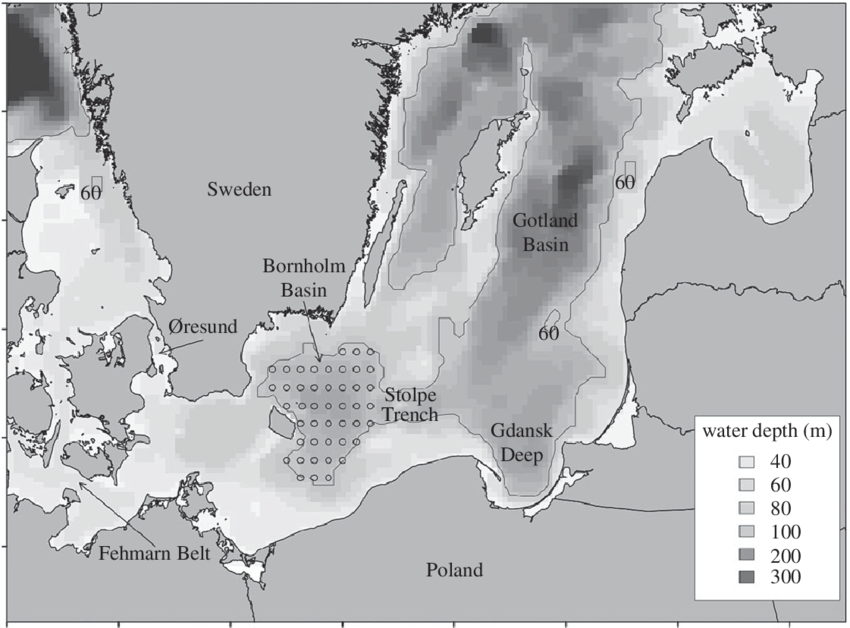
\includegraphics[width=0.5\textwidth]{Location.png}
\caption{The location of the Bornholm Basin and its water depths.\supercite{}}
\end{figure}

This study analyses some of these glider data, giving insight into two phytoplankton blooms occurring during the period March to October 2021, 
as a project part of the course MAR440 Marine Project from idea to realization at University of Gothenburg the autumn 2021.

\end{document}
